{A water tank has the shape of a truncated cone, with dimensions given below, and is filled with water with a weight density of 62.4 lb/ft$^3$. Find the work performed in pumping all water to a point 1 ft above the top of the tank.\\

\hfill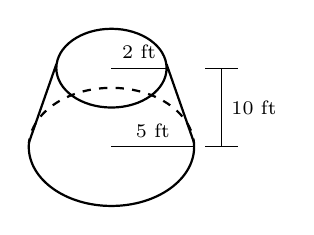
\begin{tikzpicture}[xscale=.7,yscale=.5]\draw [thick] (0,0) circle (1)
							(-1,.1) -- (-1.5,-1.9)
							(1,.1) -- (1.5,-1.9);
\draw (0,0)-- node [above,pos=.5] {\scriptsize 2 ft} (1,0)
			(0,-2) -- node [above,pos=.5] {\scriptsize 5 ft} (1.5,-2)
			(1.7,0) -- (2.3,0)
			(1.7,-2) -- (2.3,-2)
			(2,0) -- node [pos=.5,right] {\scriptsize 10 ft} (2,-2);
\draw [thick] (-1.5,-2) arc (180:360:1.5);
\draw [thick,dashed] (-1.5,-2) arc (180:0:1.5);
\end{tikzpicture}
\hfill\null
}
{187,214 ft--lb
}
